\chapter{Strategy Extraction}
\label{ch:strategy}

\newcommand{\strategyext}[0]{\textsc{strategyGen}\xspace}
\newcommand{\genstrategy}{\textsc{strategyGen}}
\newcommand{\strategy}[0]{\textsc{strategy}\xspace}
\newcommand{\partition}[0]{\textsc{partition}\xspace}
\newcommand{\nextf}[0]{\textsc{next}\xspace}
\newcommand{\ogametree}[0]{\mbox{\sc OppGT}}
\newcommand{\eagametree}[0]{\mbox{\sc AbsGT}'}
\newcommand{\pgametree}[0]{\mbox{\sc Cand}}
\newcommand{\apgametree}[0]{\mbox{\sc AbsSolvedGT}}
\newcommand{\opgametree}[0]{\mbox{\sc Spoiling}}

\newcommand{\opptf}[0]{\textsc{\textoverline{treeFormula}}}

\renewcommand{\ss}[0]{\mathbf{s}}
\newcommand{\cc}[0]{\mathbf{c}}
\newcommand{\uu}[0]{\mathbf{u}}

\newtheorem{theorem}{Theorem}
\newtheorem{example}{Example}
\newtheorem{proposition}{Proposition}

In the previous chapter I introduced an algorithm for solving realisability for bounded safety games. In most applications of synthesis it is desirable to construct a controller strategy rather than merely prove its existence. In this chapter I will introduce a strategy extraction procedure that complements the bounded reachability algorithm. This process takes abstract game trees generated during reachability analysis and, using Craig interpolation, extracts mappings of states to player actions. By using interpolation this step can be done efficiently.

The problem solved in this chapter is related to the extraction of a Skolem function for a QBF. Recall from Chapter~\ref{ch:background} that a Skolem function $f$ provides a mapping from a prefix of universal variables $\hat{y}_0, \hat{y_1}, ..., \hat{y_i}$ to existential variables $\hat{x}$ such that when substituting $\hat{x}$ for $f(\hat{y}_0, \hat{y_1}, ..., \hat{y_i})$ the QBF is equisatisfiable. A Skolem function for a bounded realisability QBF gives a mapping from a prefix of past environment actions to a controller action, i.e. a strategy for that game round. A strategy for the entire game consists of a Skolem function for every round. In this chapter, we construct a strategy by replacing the prefix of previous environment actions with a game state and current environment action pair. This allows us to solve a simpler problem than Skolemisation of the entire QBF by once again taking advantage of the structure of the bounded realisability QBF.

\section{Algorithm}

Recall that a safety game is a tuple $(\mathcal{S}, \mathcal{U}, \mathcal{C}, \delta, s_0)$ where $S$ is a set of states, $\mathcal{U}$ a set of environment action variables, $\mathcal{C}$ a set of controller action variables, $\delta$ defines a transition relation, and $s_0$ is an initial state. A set of states $E$ provides the winning condition, the controller must avoid error states and the environment must reach one. A winning strategy for controller is a function $\pi^c : 2^{\mathcal{S}} \times 2^{\mathcal{U}} \to 2^{\mathcal{C}}$ that avoids error states for the duration of the game. A controller strategy is then a mapping from state environment-action pairs to controller actions.

In this chapter we will assume that the safety game is winning for the controller. However, the technique is also easily applied to the environment to extract a spoiling strategy. In computing realisability of a safety game the algorithm constructs a \emph{certificate tree}, which is an abstract game tree $T$ such that for a set of states $s$ and game bound $\kappa$, $s \land \opptf(\kappa, \textsc{extend}(T))$ is false. In other words it is a game abstraction for which the environment has no candidate strategy.

We use the certificate tree computed by the game solver as a starting point for strategy generation.  We know that the controller can win the game in $\kappa$ rounds by picking actions from the tree; however we do not yet know which action to choose in which situation.


\subsection{Example}

Figure~\ref{fig:stratExample} introduces the running example for this chapter. It shows a state machine for a game $(\mathcal{S}, \mathcal{U}, \mathcal{C}, \delta, s_0)$ that describes the operation of a simpled clocked flip-flop. For the example we model the clock as part of the game state and assume that it oscillates in every game round. So $\mathcal{S} = \{ c, q, e \}$ is the state space of the game and contains the clock, the previous value of the flip-flop, and an error bit respectively. The environment has a single data bit variable: $\mathcal{U} = \{ d \}$ and the controller has the next value of the flip-flop: $\mathcal{C} = \{ q_n \}$. The diagram shows $\delta$ as a deterministic finite state automaton with edges labelled by a tuple $(d, q_n)$. We use $*$ as a wildcard value to simplify the presentation. The circuit described by the specification allows the environment to save a data bit $d$ into the flip-flop when the clock has a falling edge ($c$ transitions from $1$ to $0$). The controller must correctly set $q_n$ so that $q$ always contains the correct data. The initial state, $s_0$, is $c = 0 \land q = 0 \land e = 0$ and the error set is $e = 1$.

\tikzset{
    pil/.style={
        -{Latex[length=3mm]},
        thick
    },
    snode/.style={
        align=center,
        circle,
        draw,
        thick
    }
}

\begin{figure}
    \centering
    \begin{tikzpicture}
        \node [snode]
            (s1){$c = 0$ \\ $q = 0$ \\ $e = 0$};
        \node [draw=none,left=of s1] (i){};
        \node [snode,below=1.5cm of s1]
            (s0){$c = 1$ \\ $q = *$ \\ $e = 0$};
        \node [snode,right=2.5cm of s0]
            (s3){$c = 0$ \\ $q = 1$ \\ $e = 0$};
        \node [snode,accepting,right=2.5cm of s1]
            (err){$c = *$ \\ $q = *$ \\ $e = 1$};

        \draw [pil] (i) edge (s1);

        \draw [pil] (s0) edge [bend left] node [left] {$(0, 0)$} (s1);
        \draw [pil] (s1) edge [bend left] node [left] {$(*, 0)$} (s0);

        \draw [pil] (s0) edge [bend left] node [below] {$(1, 1)$} (s3);
        \draw [pil] (s3) edge [bend left] node [below] {$(*, 1)$} (s0);

        \draw [pil] (s1) edge node [above] {$(*, 1)$} (err);
        \draw [pil] (s3) edge node [right] {$(*, 0)$} (err);
        \draw [pil] (s0) edge node [above left=0mm and -3mm] {$(*, \lnot d)$} (err);
%%%        \draw [pil] (s1) edge node [below right] {$(*, 0)$} (err);
    \end{tikzpicture}
    \caption{Transition relation of the running example}
    \label{fig:stratExample}
\end{figure}

The strategy generation algorithm takes an initial set $s_0$ and its certificate tree $T$, computed by the game solver, and generates a winning controller strategy starting from $s_0$. The generated strategy must define a controller action $c \in 2^{\mathcal{C}}$ to every $\{ (s, u) \mid s \in 2^{\mathcal{S}}, u \in 2^{\mathcal{U}} \}$. The algorithm begins with $(s_0, \top)$, which it then partitions in pairs of subsets $(s_i, u_i)$, one for each outgoing branch of $T$ (Figure~\ref{fig:partition}), such that the controller can win from $s_i$ when the controller plays $u_i$ by picking action $c_i$ along the $i$th branch of the tree.  This partitioning defines the local winning strategy in the root node of $T$.  Next, for each partition $(s_i, u_i)$, the algorithm computes the set of $c_i$-successor states of $s_i$, obtaining the set $s_i'$ of states winning in the child subtree $T_i'$ of $T_i$ (Figure~\ref{fig:partition}).  The algorithm is then invoked recursively for each subtree $T_i'$.

\begin{figure}[b]
    \centering
    \captionsetup[subfigure]{width=\textwidth,justification=centering}
    \hspace*{\fill}%
    \begin{subfigure}[t]{.4\textwidth}
        \centering
        \begin{minipage}[t][3cm][t]{\textwidth}
        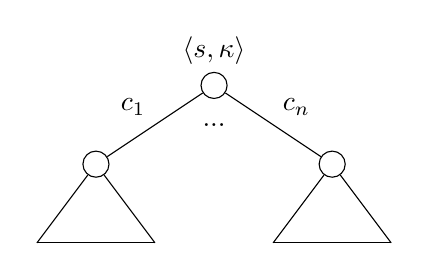
\begin{tikzpicture}[level distance = 10mm,baseline]
            \node [circle,draw] (root){}
                child {node [circle,draw] (left0){}
                    child {node (left1){}
                        edge from parent [draw=none]
                    }
                    child {node (left2){}
                        edge from parent [draw=none]
                    }
                    edge from parent node [above left] {$c_1$}
                }
                child {node [circle] {}
                    edge from parent [draw=none] node [] {$...$}
                }
                child {node [circle,draw] (right0){}
                    child {node (right1){}
                        edge from parent [draw=none]
                    }
                    child {node (right2){}
                        edge from parent [draw=none]
                    }
                    edge from parent node [above right] {$c_n$}
                }
                node [left=4pt] {}
                node [above=4pt] {$\langle s, \kappa \rangle$};

            \draw (left1.center) -- (left2.center);
            \draw (left0) -- (left1.center);
            \draw (left0) -- (left2.center);
            \draw (right1.center) -- (right2.center);
            \draw (right0) -- (right1.center);
            \draw (right0) -- (right2.center);
        \end{tikzpicture}
        \end{minipage}
        \caption{Before}
    \end{subfigure}\hfill%
    \begin{subfigure}[t]{.3\textwidth}
        \centering
        \begin{minipage}[t][3cm][t]{\textwidth}
        \begin{tikzpicture}[level distance = 10mm,baseline]
            \node [circle,draw] (root){}
                child {node [circle,draw] (left0){}
                    child {node (left1){}
                        edge from parent [draw=none]
                    }
                    child {node (left2){}
                        edge from parent [draw=none]
                    }
                    edge from parent node [left] {$c_1$}
                }
                node [above=4pt] {$\langle s_1, \kappa \rangle$};

            \node [draw=none,below right=25pt and 22pt] {$...$};

            \begin{scope}[xshift=60pt]
            \node [circle,draw] (root2){}
                child {node [circle,draw] (right0){}
                    child {node (right1){}
                        edge from parent [draw=none]
                    }
                    child {node (right2){}
                        edge from parent [draw=none]
                    }
                    edge from parent node [right] {$c_n$}
                }
                node [left=4pt] {}
                node [above=4pt] {$\langle s_n, \kappa \rangle$};
            \end{scope}

            \node [below=5pt of left0] {$T_1$};
            \node [below=5pt of right0] {$T_n$};
            \draw (left1.center) -- (left2.center);
            \draw (left0) -- (left1.center);
            \draw (left0) -- (left2.center);
            \draw (right1.center) -- (right2.center);
            \draw (right0) -- (right1.center);
            \draw (right0) -- (right2.center);
        \end{tikzpicture}
        \end{minipage}
        \caption{After}
    \end{subfigure}%
    \hspace*{\fill}
    \caption{Partitioning}
    \label{fig:partition}
\end{figure}

Figure~\ref{fig:algex} illustrates operation of the algorithm on the winning abstract game tree returned by the game solver for our running example.  Figure~\ref{fig:algexa} displays $T$, the certificate tree for the game. The algorithm starts at the root of the tree and the initial set $s = (c = 0 \land q = 0 \land e = 0)$.  The game tree defines only one winning action in the root node, hence this action is winning in all states of $s$ and no partitioning is required.  We compute the successor set reachable by playing action $q_n = 0$ in $s$: $\{ s' \mid \delta(s, \top, q_n = 0, s') \} = (c = 1 \land e = 0) $.

\tikzset{every node/.style={solid}}
\begin{figure}[b]
    \centering
    \captionsetup[subfigure]{width=\textwidth,justification=centering}
    \begin{subfigure}[t]{.4\textwidth}
        \centering
        \begin{minipage}[t][4cm][t]{\textwidth}
        \centering
        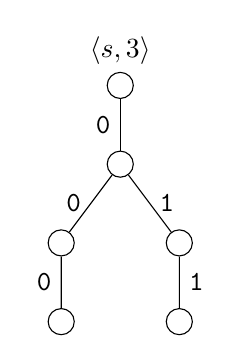
\begin{tikzpicture}[level distance = 10mm,baseline]
            \node [circle,draw] (root){}
                child {node [circle,draw] {}
                    child {node [circle,draw] {}
                        child {node [circle,draw] {}
                            edge from parent node [left] {\texttt{0}}
                        }
                        edge from parent node [left] {\texttt{0}}
                    }
                    child {node [circle,draw] {}
                        child {node [circle,draw] {}
                            edge from parent node [right] {\texttt{1}}
                        }
                        edge from parent node [right] {\texttt{1}}
                    }
                    edge from parent node [left] {\texttt{0}}
                }
                node [above=4pt] {$\langle s, 3 \rangle$};
        \end{tikzpicture}
        \end{minipage}
        \caption{$T$}
        \label{fig:algexa}
    \end{subfigure}
    \begin{subfigure}[t]{.4\textwidth}
        \centering
        \begin{minipage}[t][4cm][t]{\textwidth}
        \centering
        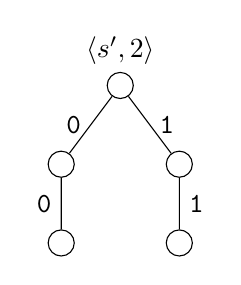
\begin{tikzpicture}[level distance = 10mm,baseline]
            \node [circle,draw] (root){}
                child {node [circle,draw] {}
                    child {node [circle,draw] {}
                        edge from parent node [left] {\texttt{0}}
                    }
                    edge from parent node [left] {\texttt{0}}
                }
                child {node [circle,draw] {}
                    child {node [circle,draw] {}
                        edge from parent node [right] {\texttt{1}}
                    }
                    edge from parent node [right] {\texttt{1}}
                }
                node [above=4pt] {$\langle s', 2 \rangle$};
        \end{tikzpicture}
        \end{minipage}
        \caption{$T'$}
        \label{fig:algexb}
    \end{subfigure}
    \begin{subfigure}[t]{.4\textwidth}
        \centering
        \begin{minipage}[t][3cm][t]{\textwidth}
        \centering
        \begin{tikzpicture}[level distance = 10mm,baseline]
            \node [circle,draw] (root1){}
                child {node [circle,draw] {}
                    child {node [circle,draw] {}
                        edge from parent node [left] {\texttt{0}}
                    }
                    edge from parent node [left] {\texttt{0}}
                };
            \node [above=4pt of root1] {$\langle s_1', 2 \rangle$};

            \node [circle,draw,right=2cm] (root2){}
                child {node [circle,draw] {}
                    child {node [circle,draw] {}
                        edge from parent node [right] {\texttt{1}}
                    }
                    edge from parent node [right] {\texttt{1}}
                };
            \node [above=4pt of root2] {$\langle s_1', 2 \rangle$};
        \end{tikzpicture}
        \end{minipage}
        \caption{AGT}
        \label{fig:algexc}
    \end{subfigure}%
    \begin{subfigure}[t]{.4\textwidth}
        \centering
        \begin{minipage}[t][3cm][t]{\textwidth}
        \centering
        \begin{tikzpicture}[level distance = 10mm,baseline]
            \node [circle,draw] (root1){}
                child {node [circle,draw] {}
                    edge from parent node [left] {\texttt{0}}
                };
            \node [above=4pt of root1] {$\langle s_1'', 1 \rangle$};

            \node [circle,draw,right=2cm] (root2){}
                child {node [circle,draw] {}
                    edge from parent node [right] {\texttt{1}}
                };
            \node [above=4pt of root2] {$\langle s_2'', 1 \rangle$};
        \end{tikzpicture}
        \end{minipage}
        \caption{$T''$}
        \label{fig:algexd}
    \end{subfigure}
    \caption{Operation of the strategy extraction algorithm on the example}
    \label{fig:algex}
\end{figure}

Next, we descend down the tree and consider subtree $T'$ and its initial set $s'$ (Figure~\ref{fig:algexb}).  We partition $(s', \top)$ into subsets $(s_1', u_1') \gets (c = 1 \land e = 0, d = 0)$ and $(s_1', u_1') \gets (c = 1 \land e = 0, d = 1)$ that are winning for the left and right subtrees of $T'$ respectively, i.e., from $(c = 1 \land e = 0)$ the controller must play action $q_n = 0$ when the environment plays $d = 0$, and $q_n = 1$ for $d = 1$.  Consider the resulting subtrees $T'_1$ and $T'_2$ with initial sets $s'_1$ and $s'_2$ (Figure~\ref{fig:algexc}).  We have $\{ s''_1 \mid \delta(s'_1, u'_1, q_n = 0, s''_1) \} = (c = 1 \land q = 0 \land e = 0)$, $\{ s''_2 \mid \delta(s'_2, u'_1, q_n = 1, s''_2) \} = (c = 1 \land q = 1 \land e = 0)$.  Finally, we obtain two subtrees $T''_1$ and $T''_2$ with initial sets $s''_1$ and $s''_2$ (Figure~\ref{fig:algexd}).  Both subtrees have one branch; hence corresponding actions $q_n = 0$ and $q_n = 1$ are winning for $(s''_1, \top)$ and $(s''_2, \top)$ respectively.

Putting together fragments of the winning strategy computed above, we obtain the following strategy for this example:
\begin{align*}
    \pi(c = 0 \land q = 0 \land e = 0, \top) &= (q_n = 0) \\
    \pi(c = 1 \land e = 0, d = 0) &= (q_n = 0) \\
    \pi(c = 1 \land e = 0, d = 1) &= (q_n = 1) \\
    \pi(c = 0 \land q = 1 \land e = 0, \top) &= (q_n = 1)
\end{align*}

The above algorithm involves two potentially costly operations: winning set partitioning and successor set computation.  If implemented na\"ively, these operations can lead to unacceptable performance.  The key insight behind our solution is that both operations can be efficiently approximated from the proof of unsatisfiability of the formula $s \land \opptf(T)$, with the help of interpolation, as described below.  The resulting approximations are sound, i.e., preserve the correctness of the resulting strategy.

\subsection{Local Strategies}

Algorithm~\ref{alg:strat} shows the pseudocode of the strategy generation algorithm.  The algorithm proceeds in two phases: the first phase (\textsc{genLocalStrats}) computes local strategies in nodes of $T$; the second phase (\textsc{compileStrat}) compiles all local strategies into a winning strategy function.

The \textsc{genLocalStrats} function recursively traverses the certificate tree $T$, starting from the root, computing local strategies in each node.  The main operation of the algorithm, called \textsc{partition}, splits $(T, s, \top)$ into $j$ tuples $(T_i, s_i, u_i)$, as shown in Figure~\ref{fig:partition}.  Each tree $T_i$ is a copy of a single branch of $T$.  The partitioning is constructed in such a way that the action $c_i$ that labels the root edge of $T_i$ is a winning controller action in $s_i$ against environment action $u_i$.

Next we consider each tuple $(T_i, s_i, u_i)$ (lines~\ref{alg:strat:for}-\ref{alg:strat:endfor}). We descend down the tree and compute the controller strategy in the child subtree $T_i'$ of $T_i$ (right-hand side of Figure~\ref{fig:partition}).  To do so, we first compute the set of $c_i$-successors of $(s_i, u_i)$: More precisely, we compute an overapproximation $\mathcal{I} \supseteq \{ s_i' \mid \delta(s_i, u_i, c_i, s_i') \}$, such that $T_i'$ is a certificate tree for $\mathcal{I}$.  Such an overapproximation is returned by the \textsc{next} function in line~\ref{alg:strat:next}.  We can now recursively invoke the strategy generation function to compute a winning strategy for the subtree $T_i'$ from $\mathcal{I}$ (line~\ref{alg:strat:rec}).

\begin{algorithm}
   \caption{Computing a winning strategy}\label{alg:strat}
   \begin{algorithmic}[1]
        \Function{GenStrategy}{$T$, $s$}
            \State $Strat \gets \Call{GenLocalStrats}{T,s}$
            \State \Return{$\Call{CompileStrat}{Strat}$}
        \EndFunction
        \Statex

        \Function{GenLocalStrats}{$T$, $s$}
            \State $[(e_1, n_1),\ldots,(e_j, n_j)] \gets \Call{succ}{T}$
            \State $[(T_1,s_1,u_1),\ldots,(T_j, s_j, u_j)] \gets \partition(T, s \land \neg E(\mathcal{S}_T))$
            \State $Strat \gets \{(s_i, u_i, \Call{action}{e_i}, \Call{height}{T}) \mid i \in[1,..,j]\}$\label{alg:strat:strati}
            \For{$i = 1$ to $j$}\label{alg:strat:for}
                \State $(T_i', s_i') \gets \nextf(T_i, s_i, u_i)$\label{alg:strat:next}
                \State $Strat_i \gets \Call{GenLocalStrats}{T_i', x_i'}$\label{alg:strat:rec}
                \State $Strat \gets Strat \cup Strat_i$
            \EndFor\label{alg:strat:endfor}
            \State \Return{$Strat$} \label{alg:strat:return}
        \EndFunction
    \end{algorithmic}
\end{algorithm}

The algorithm returns the set of tuples $(W, c, k)$.  Each tuple represents a fragment of the strategy in some tree node, where $W \in 2^{\mathcal{S}} \cup 2^{\mathcal{U}}$ is the winning set in this node, $c$ is the controller action to play in this set, and $k$ is the distance from the node to the bottom of the tree.

\subsection{Partitioning game trees}

The \textsc{partition} function (Algorithm~\ref{alg:strat:partition}) computes a local strategy in the root of an abstract game tree.  It takes a pair $(T, s)$, such that $T$ is a certificate tree for set $s$ and partitions $s$ into subsets $(s_i, u_i)$ such that the controller can win in $s_i$ when the opponent plays $u_i$ by choosing action $c_i$.

\begin{algorithm}[t]
   \caption{Partitioning winning states}\label{alg:strat:partition}
   \begin{algorithmic}[1]
        \Function{$\partition$}{$T$, $s$}
        \State $\hat{s} \gets s$
        \State $\hat{u} \gets \top$
        \State $\hat{T} \gets T$
        \For{$i = 1$ to $j$}
        \State $(T_i, \tilde{T}) \gets \Call{split}{\hat{T}}$\label{alg:partition:split}
            \State $A \gets \hat{s} \land \hat{u} \land \Call{\opptf}{\tilde{T}} $ \label{alg:strat:partition:Bi}
            \State $B \gets \Call{\opptf}{T_i} $ \label{alg:strat:partition:Ai}
            \State $\mathcal{I} \gets \Call{interpolate}{A, B}$\label{alg:partition:I}
            \State $(s_i, u_i) \gets (\mathcal{I}(\mathcal{S}_T) \land \hat{s}, \mathcal{I}(\mathcal{U}_T) \land \hat{u})$\label{alg:partition:Ii}
            \State $\hat{s} \gets \hat{s} \land \neg s_i$
            \State $\hat{u} \gets \hat{u} \land \neg u_i$
            \State $\hat{T} \gets \tilde{T}$\label{alg:partition:upd}
        \EndFor
        \State \Return{$[(T_1, s_1, u_1),\ldots, (T_j, s_j, u_j)]$} \label{alg:strat:partition:return}
        \EndFunction
    \end{algorithmic}
\end{algorithm}

At every iteration, the algorithm splits the tree into the leftmost branch $T_i$ and the remaining tree (Figure~\ref{fig:split}).  It then computes the pair $(s_i, u_i)$ where the controller wins by following the branch $T_i$, removes $s_i$ from the initial set $s$, and $u_i$ from the set of opponent moves $u$.  At the next iteration it considers the leftover tree $\tilde{T}$ and shrunk initial sets $\hat{s}$ and $\hat{u}$.

\begin{figure}
    \centering
    \begin{tikzpicture}[level distance = 12mm,baseline]
        \node [circle,draw] (root){}
            child {node [circle,draw] (left0){}
                child {node (left1){}
                    edge from parent [draw=none]
                }
                child {node (left2){}
                    edge from parent [draw=none]
                }
                edge from parent node [below left=-1mm and 3mm] {$c_i$}
            }
            child {node [circle,draw,right=8mm] (leftb0){}
                child {node (leftb1){}
                    edge from parent [draw=none]
                }
                child {node (leftb2){}
                    edge from parent [draw=none]
                }
                edge from parent node [below right=-1mm and 2mm] {$c_{i+1}$}
            }
            child {node [circle,draw,right=11mm] (leftc0){}
                child {node (leftc1){}
                    edge from parent [draw=none]
                }
                child {node (leftc2){}
                    edge from parent [draw=none]
                }
                edge from parent node [below right=-1mm and 5mm] {$c_{j}$}
            }
            node [above=4pt] {$\langle x_0, \kappa \rangle$};


        \node [draw,
            dash pattern=on 2pt off 2pt,
            minimum width=6.5cm,
            minimum height=4cm,
            below right=-10mm and -27mm
            ] {};
        \node [above=8mm of root] (startline) {};
        \node [below=29mm of root] (endline) {};
        \draw [dash pattern=on 2pt off 2pt] (startline) -- (endline);

        \node [below=5pt of left0] {$T_i$};
        \node [below=5pt of leftb0] {$T_{i+1}$};
        \node [below=5pt of leftc0] {$T_j$};
        \draw (left1.center) -- (left2.center);
        \draw (left0) -- (left1.center);
        \draw (left0) -- (left2.center);
        \draw (leftb1.center) -- (leftb2.center);
        \draw (leftb0) -- (leftb1.center);
        \draw (leftb0) -- (leftb2.center);
        \draw (leftc1.center) -- (leftc2.center);
        \draw (leftc0) -- (leftc1.center);
        \draw (leftc0) -- (leftc2.center);
        \node [right=4mm of leftb0] {...};
        \node [above=6mm of left0] {$(T_i, x_i)$};
        \node [above=6mm of leftc0] {$(\tilde{T}, \hat{x} \setminus x_i)$};
    \end{tikzpicture}
    \caption{Splitting of $T$ in the \textsc{Partition} function.\label{fig:split}}
\end{figure}

The algorithm maintains the invariant that $\hat{T}$ is a certificate tree for $\hat{s}$ if the environment chooses from $\hat{u}$, and hence $\hat{s} \land \hat{u} \land \opptf(\hat{T})$ is unsatisfiable.  We decompose this formula into two conjuncts $A \land B$ such that $A$ and $B$ only share state and action variables $\mathcal{S}_T \cup \mathcal{U}_T$ in the root node of $T$ and that the interpolant $\mathcal{I}$ of $A$ and $B$ consists of states and environment actions for which the controller can win by following the $T_i$ subtree.  Hence $(\mathcal{I}(\mathcal{S}_T) \land \hat{s}, \mathcal{I}(\mathcal{U}_T) \land \hat{u})$ gives us the desired pair $(s_i, u_i)$.  

Informally, $A$ is a partial expansion of the game formula induced by $\tilde{T}$.  It is satisfiable iff there exists a spoiling environment strategy from $\hat{s}$ and allowable by $\hat{u}$ against abstract game tree $\tilde{T}$.  $B$ is a partial expansion of the game induced by $T_i$.  It is satisfiable iff there exists a spoiling environment strategy against $T_i$.  Both $A$ and $B$ can be satisfiable individually, but because $T$ is a certificate tree their conjunction is unsatisfiable.

The interpolant $\mathcal{I}$ of $A$ and $B$ implies $\neg B$, i.e., for any state and environment action in $\mathcal{I}$, $c_i$ is a winning move.  $\mathcal{I}$ is also implied by $A$, i.e., it contains all states in $s$ and all environment actions for which the controller cannot win by picking moves from $\tilde{T}$ as a subset.  Equivalently, for any state in $\hat{s} \land \neg \mathcal{I}(\mathcal{S}_T)$ and environment action in $\hat{u} \land \neg \mathcal{I}(\mathcal{U}_T)$, the controller \emph{can} win by following $\tilde{T}$, i.e., $\tilde{T}$ is a certificate tree for ($\hat{s} \land \neg \mathcal{I}(\mathcal{S}_T), \hat{u} \land \neg \mathcal{I}(\mathcal{U}_T))$, and we can apply the decomposition again to $\tilde{T}$ at the next iteration.


\makeatletter
\newcommand{\pushright}[1]{\ifmeasuring@#1\else\omit\hfill$\displaystyle#1$\fi\ignorespaces}
\makeatother

We prove useful properties of the $\partition$ function. We begin with the proposition that $A$ and $B$ imply a decomposition of $\hat{s} \land \hat{u} \land \opptf(\hat{T})$. 
\begin{proposition}\label{prop:aandb}
    $A\land B \implies \hat{s} \land \hat{u} \land \opptf(\hat{T})$.
\end{proposition}
\begin{proof}
    \begin{align*}
        A \land B ={}& (\hat{s} \land \hat{u} \land \opptf(\tilde{T})) \land \opptf(T_i) \\
        A \land B ={}& \hat{s} \land \hat{u} \land \bigg( E(\mathcal{S}_{\tilde{T}}) \lor \\
                     & \pushright{ \bigvee_{\langle e, n \rangle \in \textsc{succ}(\tilde{T})} \delta(\mathcal{S}_{\tilde{T}}, \mathcal{U}_{\tilde{T}}, \mathcal{C}_{\tilde{T}}, \mathcal{S}_n) \land \textsc{action}(e) \land \opptf(n) \bigg)} \\
                     & \pushright{\land \bigg( E(\mathcal{S}_{T_i}) \lor (\delta(\mathcal{S}_{T_i}, \mathcal{U}_{T_i}, \mathcal{C}_{T_i}, \mathcal{S}_{n_i}) \land \textsc{action}(e_i) \land \opptf(n_i)) \bigg)} \\
        \implies{}& \hat{s} \land \hat{u} \land \bigg( E(\mathcal{S}_{\hat{T}}) \lor \\
                  & \pushright{  \bigvee_{\langle e, n \rangle \in \textsc{succ}(\hat{T})} \delta(\mathcal{S}_{\hat{T}}, \mathcal{U}_{\hat{T}}, \mathcal{C}_{\hat{T}}, \mathcal{S}_n) \land \textsc{action}(e) \land \opptf(n) \bigg)} \\
        ={}& \hat{s} \land \hat{u} \land \opptf(\hat{T})
    \end{align*}
\end{proof}

\begin{proposition}
    The following invariant is maintained throughout the execution of \textsc{partition}: $\hat{T}$ is a certificate tree for $\hat{s}$ when the environment may choose actions from $\hat{u}$.
\end{proposition}
\begin{proof}
    We prove by induction. It is a precondition of the function that $T$ is a certificate tree for $s$, thus the invariant holds for the initial values of $\hat{T} = T$, $\hat{s} = s$, and $\hat{u} = \top$.  By the induction hypothesis $(\hat{s} \land \hat{u} \land \opptf(\hat{T}))$ is unsatisfiable, so by Proposition~\ref{prop:aandb} $(A \land B)$ must also be unsatisfiable.  Hence the interpolation operation in line~\ref{alg:partition:I} is well defined.  By the properties of interpolants, $(A \implies \mathcal{I})$, hence $(\neg \mathcal{I} \implies \neg A)$ or equivalently $(\neg\mathcal{I} \implies \neg (\hat{s} \land \hat{u} \land \opptf(\tilde{T}))$.

    After $\hat{T}$, $\hat{s}$, and $\hat{u}$ are updated in line~\ref{alg:partition:upd}, their new values $\hat{T}'$, $\hat{s}'$, and $\hat{u}'$ satisfy the following equalities: \begin{align*}
        \hat{s}' \land \hat{u}' \land \opptf(\hat{T}') ={}& \hat{s} \land \hat{u} \land \opptf(\tilde{T}) \land \neg\mathcal{I} \\
        ={}& \neg\mathcal{I} \land \hat{s} \land \hat{u} \land \opptf(\tilde{T}) \\
        \implies{}& \neg (\hat{s} \land \hat{u} \land \opptf(\tilde{T})) \\
                  & \pushright{\land \hat{s} \land \hat{u} \land \opptf(\tilde{T})} \\
        ={}& \bot
\end{align*} and hence the invariant is maintained.
\end{proof}

\begin{proposition}\label{prop:partition}
    Let $T$ be a certificate tree for $s$ and let $s \land \lnot E(\mathcal{S}_T) = \bot$. Then $[(T_1, s_1, u_1),\ldots,(T_j, s_j, u_j)] = \textsc{partition}(T, s)$ is a local winning strategy in the root of $T$, i.e., the following properties hold:
    \begin{enumerate}
        \item Sets $(s_1,u_1) ,\ldots, (s_j,u_j)$ comprise a partitioning of
            $(s, \top)$: $s = \bigvee s_i$, $\top = \bigvee u_i$ and $\forall i, k. (i\neq k) \implies (s_i \land u_i) \land (s_k \land u_k) = \bot$
        \item $T_i$ is a certificate tree for $s_i$ under environment actions $u_i$, for all $i\in[1,j]$
    \end{enumerate}
\end{proposition}
\begin{proof}
    At every iteration of the algorithm, we partition $\hat{s}$ into $s_i = \mathcal{I}(\mathcal{S}_T) \land \hat{s}$ and $\hat{s} \land \neg\mathcal{I}(\mathcal{S}_T)$. We do the same for $\hat{u}$: $u_i = \mathcal{I}(\mathcal{U}_T) \land \hat{u}$ and $\hat{u} \land \neg\mathcal{I}(\mathcal{U}_T)$. Hence the different sets in each $s_i$ and $u_i$ do not overlap by construction.

    At the final iteration of the algorithm, the tree $\tilde{T}$ consists of a single root node without outgoing branches.  Hence, $A = \hat{s} \land \hat{u} \land \opptf(\tilde{T}) = \hat{s} \land \hat{u} \land \neg E(\mathcal{S}_{\tilde{T}}) = \hat{s} \land \hat{u}$.  Since $(A \implies \mathcal{I})$, we get $((\hat{s} \land \hat{u}) \implies \mathcal{I})$ and therefore $\mathcal{I} \land \hat{u} \land \hat{s} = \hat{s} \land \hat{u}$, i.e., all states in $\hat{s}$ and $\hat{u}$ are included in the final pair $(s_j, u_j)$ and hence the partitioning completely covers sets $(s, \top)$: $s=\bigvee s_i$ and $\top = \bigvee u_i$.

    We prove the second statement of the proposition.  The sets $s_i$ and $u_i$ are computed as
    $\mathcal{I}(\mathcal{S}_T) \land \hat{s}$ and $\mathcal{I}(\mathcal{U}_T) \land \hat{u}$ at the $i$th iteration of the algorithm (line~\ref{alg:partition:Ii}).
    Thus, 
    \begin{align*}
        s_i \land u_i \land \opptf(T_i) ={}& \mathcal{I}(\mathcal{S}_T) \land \hat{s} \land \mathcal{I}(\mathcal{U}_T) \land \hat{u} \land \opptf(T_i) \\
        ={}& \mathcal{I} \land \hat{s} \land \hat{u} \land \opptf(T_i)
    \end{align*}
    By the properties of interpolants, $\mathcal{I} \land B = \mathcal{I} \land \opptf(T_i) = \bot$.
    Hence $s_i \land u_i \land \opptf(T_i) = \bot$, i.e., $T_i$ is a certificate tree for $s_i$ under opponent actions $u_i$.
\end{proof}

\subsection{Determine an action}

The \textsc{next} function (Algorithm~\ref{alg:next}) takes a set $s$, a set $u$, and its certificate tree $T$, such that there is exactly one outgoing edge, labelled $c$, from the root node of $T$.  $T$ has a sole child subtree $T'$ with root node $n$.  The function computes an overapproximation $s'$ of the $c$-successor of ($s$, $u$), such that $s'$ is winning for the controller and $T'$ is a certificate tree for $s'$.

\begin{algorithm}
   \caption{Successor set}\label{alg:next}
   \begin{algorithmic}[1]
        \Function{$\nextf$}{$T, s, u$}
        \State $[(e, n)] \gets \Call{succ}{T}$ \Comment{$T$ has a single successor}
            \State $A \gets s \land u \land \delta(\mathcal{S}_T, \mathcal{U}_T, \mathcal{C}_T, \mathcal{S}_{n}) \land \Call{action}{e}$\label{alg:strat:partition:Ai}
            \State $B \gets \opptf(n) $\label{alg:strat:partition:Bi}
            \State $\mathcal{I} \gets \Call{interpolate}{A, B}$ \label{alg:strat:partition:I}
            \State \Return{$(n, \mathcal{I}(\mathcal{S}_{n}))$} \label{alg:strat:partition:return}
        \EndFunction
    \end{algorithmic}
\end{algorithm}

Once again, we decompose the unsatisfiable formula $s \land u \land \opptf(T)$ into two conjuncts $A$ and $B$.  $A$ encodes one round of the game from the set $s$ under $u$, where the controller plays action $c$.  $B = \opptf(T')$ is a partial $\forall$-expansion of the game induced by $T'$.  $A$ and $B$ only share state variables $\mathcal{S}_{n}$ (where $n$ is the root node of $T'$ and single successor node of $T$) and their interpolant gives the approximation we are looking for.

\begin{proposition}\label{prop:next}
    Let $T$ be a certificate tree for $s$ under opponent actions $u$ with a single outgoing edge, labelled $c$ in its root node, and let $(T',\mathcal{I})
    = \textsc{next}(T,s,u)$.
    Then:
    \begin{enumerate}
        \item $\mathcal{I}$ is an overapproximation of the $c$-successor of $s$ under $u$, i.e., $$\mathcal{I} \supseteq \{ s' \mid \delta(s, u, c, s') \}$$
        \item $T'$ is a certificate tree for $s'$
    \end{enumerate}
\end{proposition}
\begin{proof}
    The $c$-successor set $s'$ of $s$ under environment actions $u$ is defined by $\exists s_T, u_T (s \land u \land \delta(s_T, u_T, c_T, s') \land c_T = c)$. The matrix of this formula is exactly formula $A$.  Hence the successor set is given by $s' = \exists s_T,u_T (A)$.  Since $(A \implies \mathcal{I})$, $s' \implies \exists s,u.  \mathcal{I}$.  Since $\mathcal{I}$ is defined over state variables in the root of $T'$ only, the quantifiers can be removed: $s' \implies \mathcal{I}$ or, in the relational form, $\mathcal{I} \supseteq s'$.
    
    We prove the second property by the construction of the interpolant: $(\mathcal{I} \land \opptf(T')) = (\mathcal{I} \land B) = \bot$.
\end{proof}

\subsection{Compiling the strategy}

Finally, we describe how local strategies computed by \textsc{genLocalStrats} are combined into a winning strategy for the game.  This requires some care, as individual partial strategies can be defined over overlapping sets of states.  We want the resulting strategy function to be deterministic; therefore for each partial strategy we only add new states not yet covered by the computed combined strategy.  Function \textsc{compileStrats} (Algorithm~\ref{alg:compile}) achieves this by keeping track of all states $W$ already added to the strategy.  For every new tuple $(w, a, k)$, it restricts the set $w$ to $\neg W$, which guarantees that no state action pair can be added to the strategy twice.  

%%%Furthermore, by considering tuples with smaller values of $k$ first, we resolve the nondeterminism.

\begin{algorithm}[t]
   \caption{Compiling the  winning strategy}\label{alg:compile}
   \begin{algorithmic}[1]
        \Function{CompileStrat}{$Strat$}
            \State $\pi \gets \bot,~~W \gets \bot$
            \For{$(w, c, k) \in Strat$} %\Comment{Sorted by ascending $k$}
            \State $\pi \gets \pi \lor (w \land \neg W \land (\mathcal{C}=c))$
                \State $W \gets W \lor w$
            \EndFor
            \State \Return $\pi$
        \EndFunction
    \end{algorithmic}
\end{algorithm}

%%%Let $\textsc{rank}(s, u), s \in \mathcal{S}, u \in \mathcal{U}$, be the smallest $k$ such that there exists $(w,c,k) \in Strat$, $s \land u \in w$, or $\infty$ if there is no such $k$.

%%%\begin{proposition}\label{prop:rank}
%%%    Let $\pi=\textsc{compileStrat}(Strat)$. For any triple $(s, u, c) \in \pi$, there exists $(w, c, k) \in Strat$ such that $s \land u \in w$ and $k=\textsc{rank}(s, u)$.
%%%\end{proposition}

%%%\begin{theorem}[Correctness of the algorithm]
%%%Let abstract game tree $T$ of height $\kappa$ be a certificate tree for the set $s$, let $\pi$ be a partial function returned by the strategy generation algorithm, $\pi=\textsc{genStrategy}(T,s)$, and let $\pi'$ be an arbitrary extension of $\pi$ to a complete function.  Then $\pi'$ is a winning controller strategy of length $\kappa$ from $s$.
%%%\end{theorem}
%%%\begin{proof}
%%%    Every tuple $(s, u, c)$ in $\pi$ is generated by the \textsc{partition} function and, according to Proposition~\ref{prop:partition}, $c$ is a winning controller move in $s$ under environment action $u$. By Proposition~\ref{prop:next}, all possible $c$-successors of $(s, u)$ are covered by $\pi$.  Hence, by following the strategy $\pi$ from $I$, the controller is guaranteed to stay within the safe region of the game until reaching the bound.

%%%Next, we show that ranks of states visited by following the
%%%strategy $\pi$ decrease monotonically and hence the strategy
%%%reaches the goal in at most $n$ steps. According to
%%%Proposition~\ref{prop:rank}, for every pair $(s,a) \in \pi$, there
%%%exists $(I, a, k)\in Strat$, such that $k=rank(s)$.  Therefore,
%%%for any $s'\in succ(s,a)$, such that $s'\not\in O$, there exists
%%%$(I', a', k-1)\in Strat$, $s'\in I'$; hence $rank(s')\leq k-1 < k
%%%= rank(s)$.
%%%\qed
%%%\end{proof}

\section{Related work}

All existing strategy extraction algorithms for games were developed for use with game solvers based on winning set compilation~\cite{Bloem14}.  Such a solver generates a sequence of expanding state sets for which the game is safe for $1,2,\ldots$ steps.  The task of the strategy extraction algorithm is to compute a function that in every winning state chooses a single move that forces the game back into a safe state.  In contrast, our strategy generation algorithm does not require the game solver to compile winning regions, but instead uses abstract game trees.

Another line of related work is strategy extraction algorithms for QBF used in QBF certification. QBF strategy extraction methods are specific to the underlying proof system used by the QBF search algorithm~\cite{Lonsing10,Egly13,Goultiaeva11}.  A strategy in a QBF is an oracle that, given the history of moves played in the game, outputs the next move for the winning player.  An additional procedure is required to convert this oracle into a memory-free strategy function that maps a state to a controller move.  Our work can been seen as such a procedure for $\forall Exp+Res$ proof system based solvers~\cite{Janota13}.

\section{Summary}

I have presented a strategy extraction algorithm to extended bounded realisability to bounded synthesis. The algorithm assigns controller actions to pairs of states and environment actions by a lightweight recursive application of interpolation to the certificate tree generated by the game solver. The performance overhead of this approach will be evaluated in Chapter~\ref{ch:evaluation}.
